\section{Code}
\subsection{Payload} \label{app:code_payload}
The follow code contains functions used by the OBC to perform the voltage sweep and analyse the data.

\lstinputlisting[style=CStyle]{code/payload/LP_functions.ino}

\subsection{Attitude Determination and Control \label{app:mat}}

\subsubsection{Main code}

\lstinputlisting{code/adcs/main_display.m}

\subsubsection{Satellite Dynamics: \texttt{satDyn.m}}

\lstinputlisting{code/adcs/satDyn.m}

\subsubsection{ADCS Loop: \texttt{adcs.m}}

\lstinputlisting{code/adcs/adcs.m}

\subsubsection{Unscented Kalman Filter: \texttt{UKF.m}}

\lstinputlisting{code/adcs/UKF.m}

\subsubsection{Controllers: \texttt{controlLQR.m}}

\lstinputlisting{code/adcs/controlLQR.m}

\section{Link Calculations \label{app:LinkCalc}}
The following values are typical for this type of system, and have been derived from research: bit error rate $<10^-5$, LNA noise temperature $T_{down}=50K, T_{up}=289K$, spacecraft transmission line temperature $T_{trans, sat} = 51.2K$ demodulation implementation loss $3dB$, threshold $E_{b}/N_{0}=9.6dB$ \cite{SMAD}, ground station transmission line loss $3.29dB$ \cite{LineLossGS}, loss due to rain/snow $0dB$, ionospheric loss $0.1dB$ \cite{RainLoss}, atmospheric loss $1dB$ \cite{AtmosLoss}, transponder intermodulation ratio $IMR=50dB$, per used channel bandwidth $BW_{user}=air data rate/2=4kbps$, spacecraft sky temperature $T_{sky, down}=90K$, $T_{sky, up}=290K$ \cite{SMAD}, antenna polarisation loss $L_{pol}=-3dB$ and the transponder uplink interference density $\rho_{int, up}=-250dbW/Hz$.

\subsection{Slant Range}
The slant range is the measure of the maximum distance between the satellite and the groundstation, and will be used to later find the free-space loss.
It can simply be found using geometry, the elevation angle of the satellite and it's altitude. The altitude for the chosen orbit is $400$km, and the elevation angle is $35^o$. We need a minimum of $20^o$ to be visible by the earth at all, to which we add the $5^o$ for visibility.
\begin{equation}
slant range = \dfrac{altitude}{sin(\theta_{el})}=697.38km
\end{equation}

\subsection{Pointing Loss}
The pointing loss is loss associated with the antenna of the satellite not being accurately pointed at the ground station and vice versa. Due to the high velocity of the satellites this is easily possible, and they can be found using the following formula.
\begin{equation}
pointing loss = \frac{12\alpha_{T}}{\theta_{3dB}}=1dB_{Dipole}, 3dB_{Yagi}
\end{equation}
Where the angle of misalignment has been chosen to be $\alpha_{T}=8.4^o$, and the $\theta_{3dB}$, the beam width at half power is $80^o$ and $50^o$ \cite{BeamWidth} for the dipole and the yagi-type antenna respectively.

\begin{landscape}
		\clearpage\pagestyle{empty} 
\subsection{Power Budget}
	\begin{figure}[H]
		\centering
		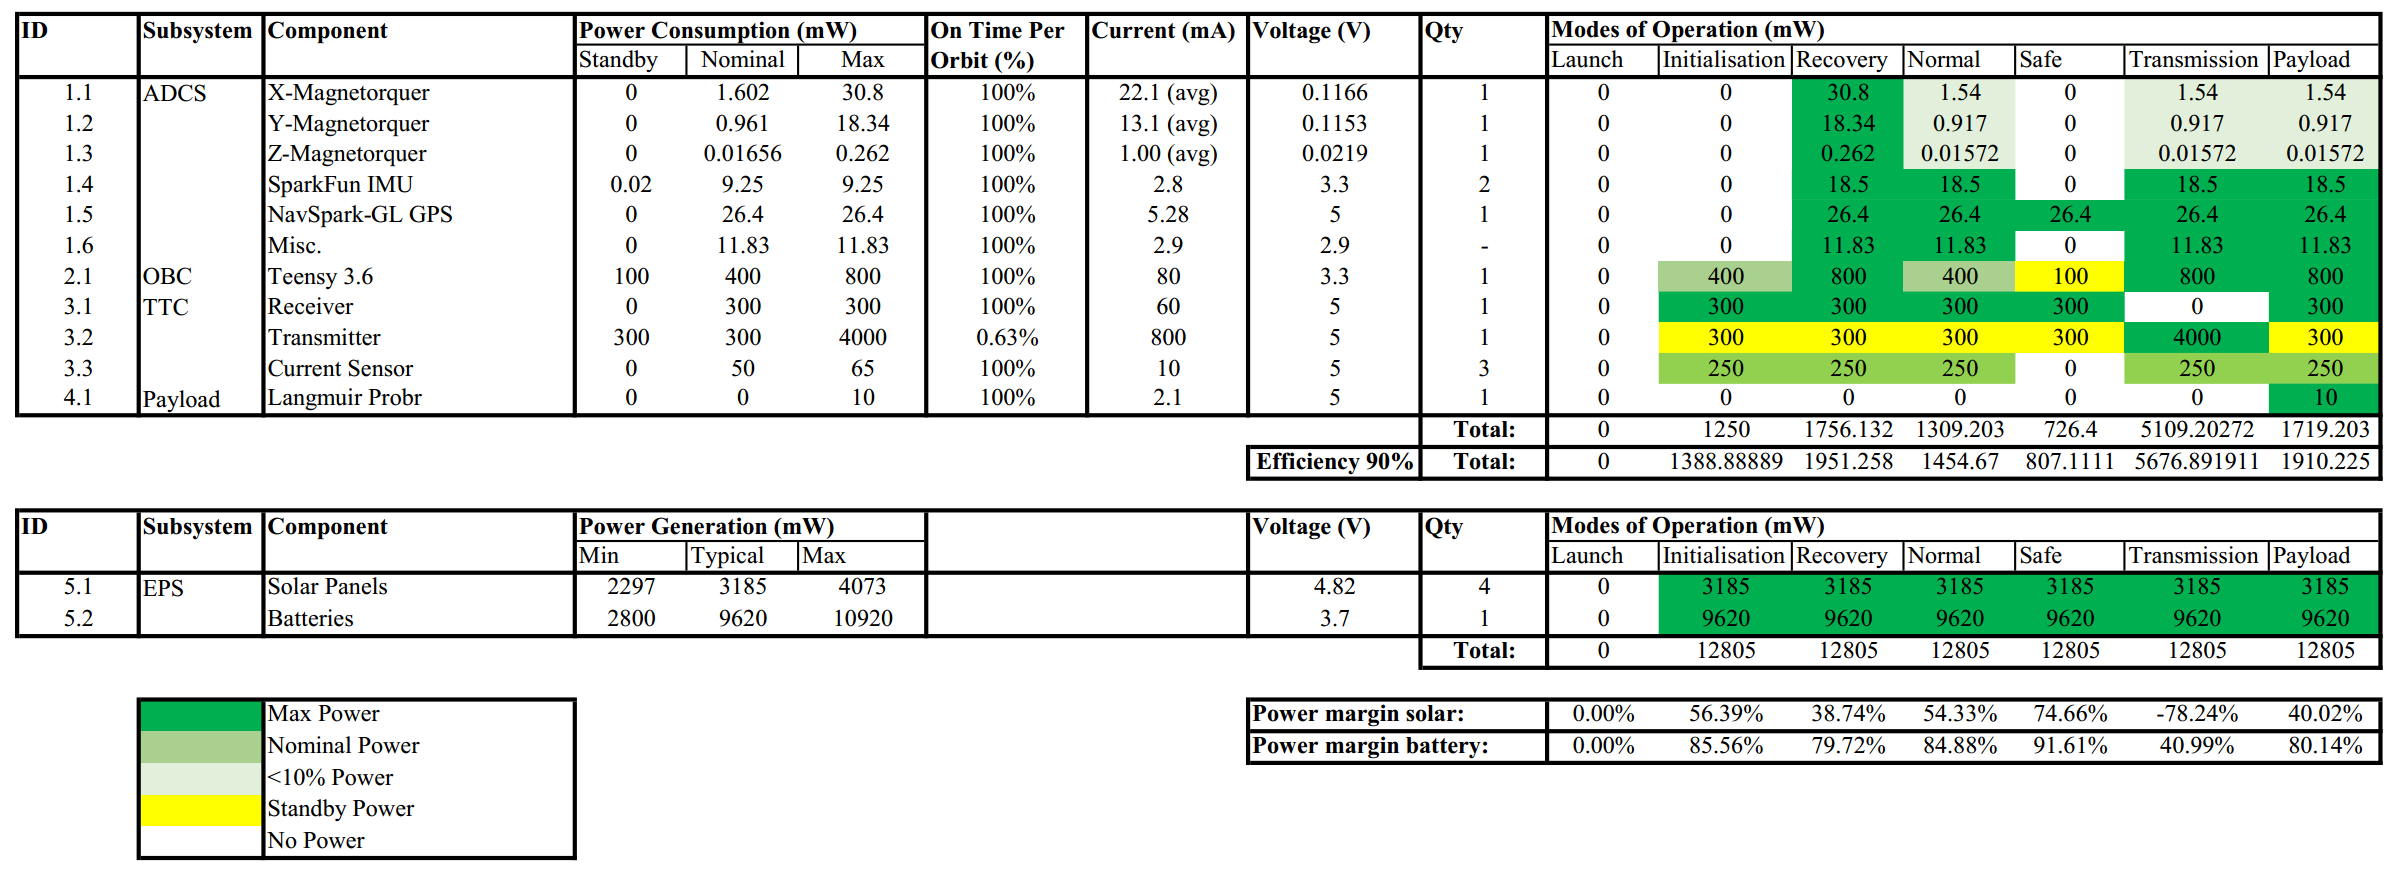
\includegraphics[scale=0.8]{power_budget}
		\caption{Power budget}
		\label{fig_pwrBud}
	\end{figure}
\end{landscape}

\subsection{EIRP}
The effective isotropic radiated power is a simple measure of an antennas radiated power, by assuming it's an isotropic radiator\cite{SMAD}.
This measure can be found by adding the transmitter power, with the antenna gain and taking away the transmission line losses, when working in dB.
\begin{equation}
EIRP=P_{T}+G_{A}-L_{T}
\end{equation}

\subsection{Free Space Loss}
The free space loss is the largest part of the power loss, and it occurs over the distance the signal has to travel through free space. It is calculated the following formula, where $R$ is the slant range, $f$ is the frequency of transmission in Hz, and $c$ is the speed of light.

\begin{equation}
FSPL=(\frac{4\pi Rf}{c})^2
\end{equation}

\subsection{Figure of Merit}
Figure of merit is a measure of how the gain of the antenna compares to the noise in the system. It can be found using the gain of the antenna $G_{A}$ and the system noise temperature $T_{s}$, both in decibels.
\begin{equation}
FoM=G_{A}-T_{s}
\end{equation}

\subsection{Carrier Power}
The carrier power is a measure of the energy of the carrier signal. This means it is simply the sum of all gains and losses with the EIRP.

\begin{equation}
C=EIRP+G-L
\end{equation}

\subsection{Noise Density}
As we can see the carrier power is relatively small, but due to the system set-up, so is the noise density. This can be found by converting the noise temperature to an amplitude in decibels, using Boltzmann's constant.

\begin{equation}
N_0=k_{b, dB}+T_{s}
\end{equation}

\subsection{Carrier Power to Noise Density Ratio}
This ratio is relatively self-explanatory, as it expresses the ratio between the strength of the signal to the noise present. It can be found using
\begin{equation}
C-N ratio=\dfrac{C}{N_{0}}
\end{equation}


\subsection{$E_{b}/N_{0}$}
This measure is closely related to the C-N ratio, but instead of the total power it gives the energy per bit, compared to the noise density. To get this value, we simply need to divide by the data-rate $R_b$ chosen.
\begin{equation}
E_{b}/N_{0}=\frac{C}{N_{0}}-10\log(R_b)=20.02dB_{up}, 16.75dB_{down}
\end{equation}

The combined ratio is given to be $15.07dB$. Every modulation technique has a threshold value, under which the noise will be too large to decipher the original signal. For the chosen method this limit is $9.6dB$.\\

This then leaves a system link margin of $10.42dB$ for uplink and $7.15dB$ for downlink in the link performance.

\section{Detailed Mass Budget}

\begin{landscape}
	\clearpage\pagestyle{empty} 
	\begin{figure}[H]
		\centering
		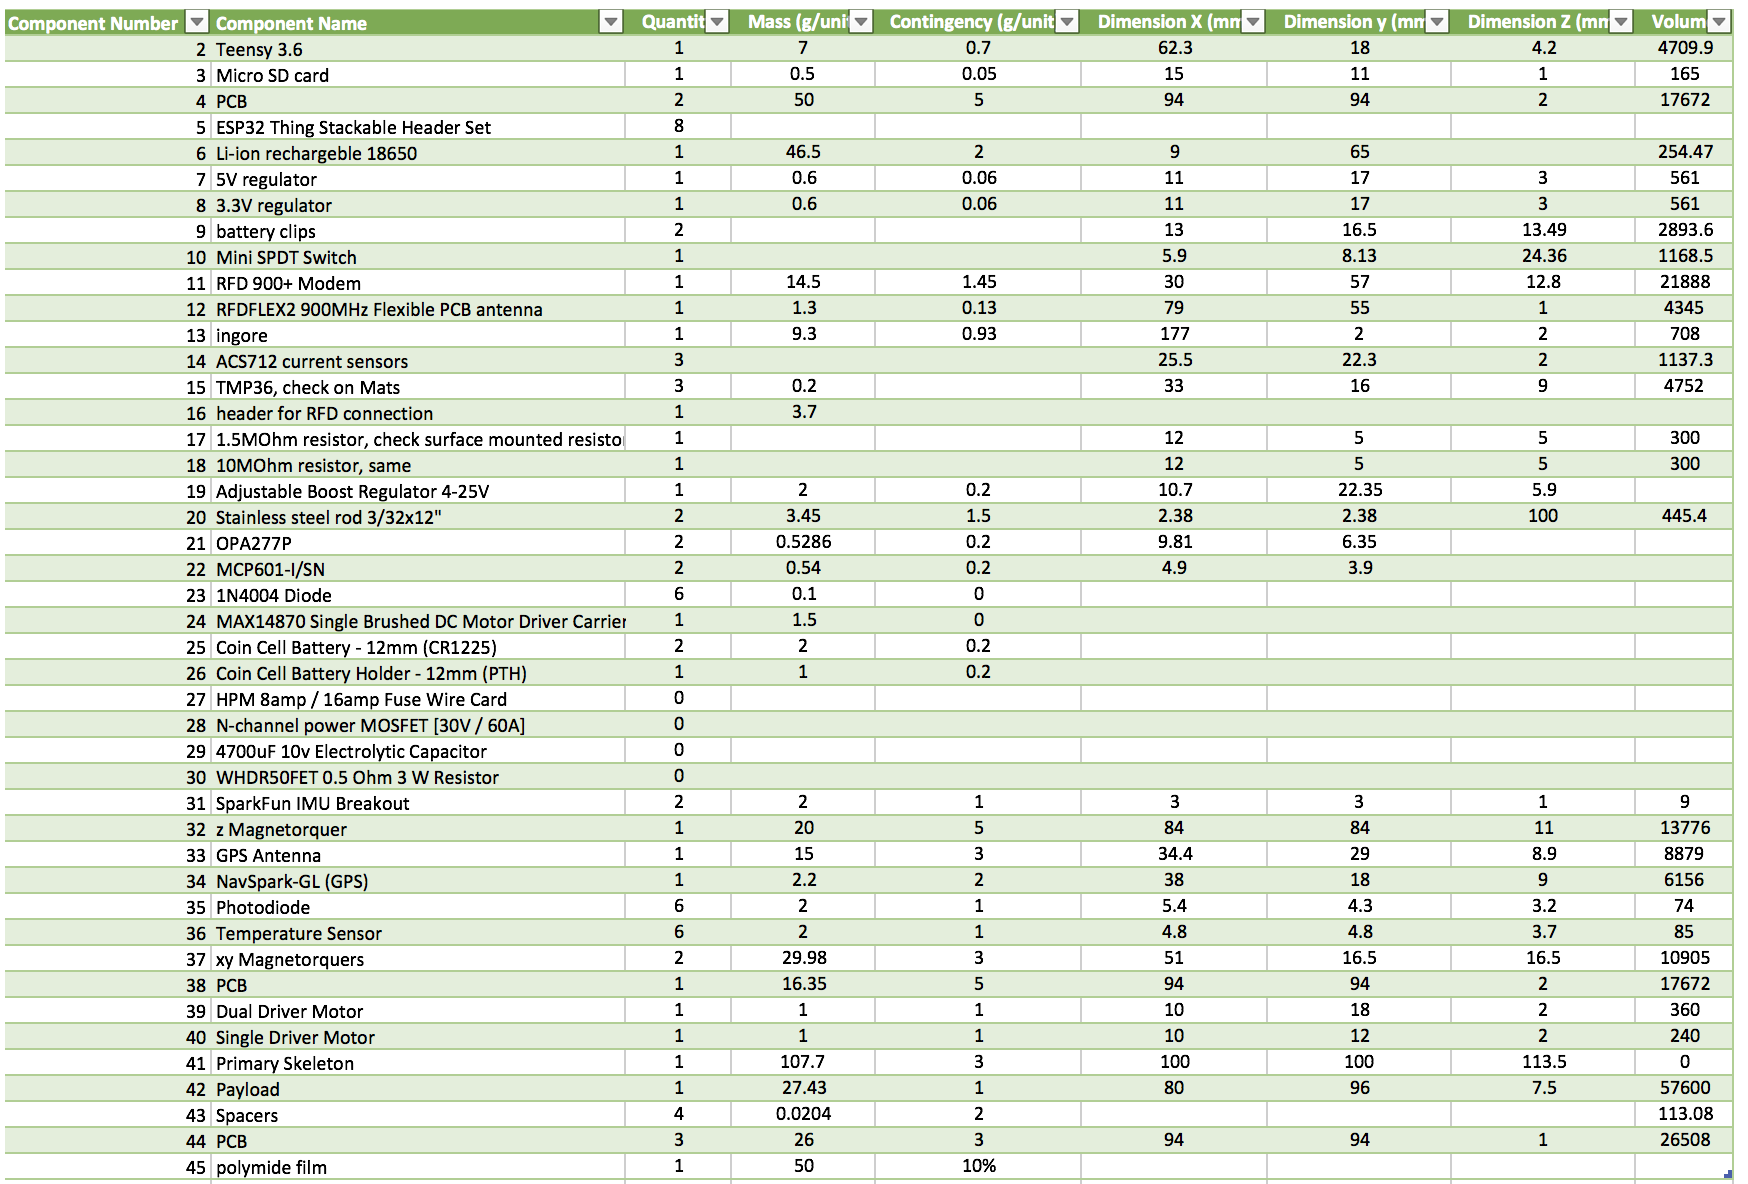
\includegraphics[scale=0.7]{MassBudgie}
		\caption{Mass Budget}
		\label{MassBudgie}
	\end{figure}
\end{landscape}
